\chapter{Technical design}
\label{chap:techdesign}

\section{Operating system}

Since Microsoft Windows and Apple MacOS are not open source operating systems, they cannot be considered as a basis for Hellonium.

Due to the author's insufficient experience with BSD, it was not considered.

The author has been able to gather extensive experience with GNU/Linux for over 20 years. On the server side he has favoured Debian GNU/Linux for years and on the client side he currently favours Arch Linux.

Due to a major change in the Debian project regarding the creation of live systems for optical media, the process is currently somewhat easier under Arch Linux with the \glqq{}archiso\grqq{}\footnote{https://wiki.archlinux.de/title/Archiso} tool.

Until the development is completed, an external SSD can be used with Arch Linux.

\section{Software}

Since Debian GNU/Linux is rather conservative in terms of package versions and only releases a new version about every two years, Arch Linux was given preference. It has been shown that up-to-date software is necessary, especially for MacOS guests. Arch Linux follows the rolling release and is thus always very up-to-date.

Basically all necessary tools are available as packages for Arch Linux.

Should this not be the case, own recipes can be made available via the Arch Linux User Repository (AUR).

Only in exceptional cases should internal software solutions be used. However, these must not be published via AUR as a matter of principle.

\section{GUI}

User-friendliness already begins with the graphical desktop. This should be preconfigured as well as possible for the intended use.

Since an independent development of a GUI would have exceeded the time frame of the thesis, the possibility was chosen to supplement the file manager Nautilus from the Gnome project with scripts. In order not to have to fulfil any unnecessary dependencies and to ensure the most error-free integration of the file manager possible, the choice of the desktop interface fell on Gnome. The development took place under version 3. However, initial tests have not revealed any problems with version 4.

\begin{figure}[htbp]  % order of priority: h here, t top, b bottom, p page
  \centering
  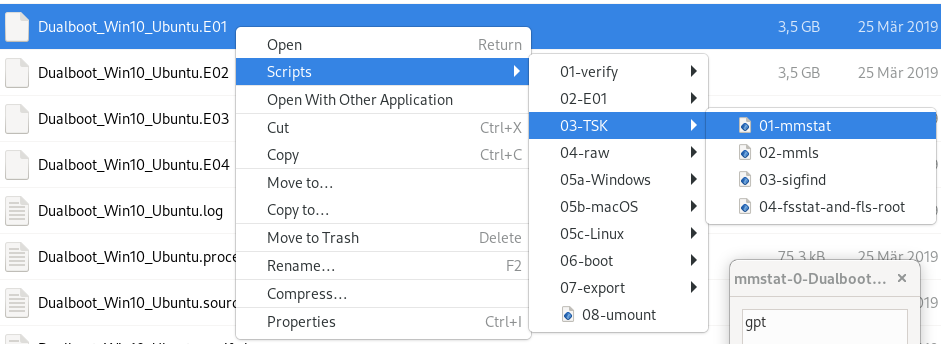
\includegraphics[width=.5\textwidth]{figures/mmstat-gpt.png}
  \caption[Nautilus script example]{The screenshot shows a nautilus script to get the partition scheme.}
  \label{fig:NautilusScript}
\end{figure}

As can be seen in \cref{fig:NautilusScript} , after right-clicking on an EWF\_E01 image, one can select the later functionalities of Hellonium under Scripts.

In the implementation phase, the goal is to find or package the right tools and make them easy to use via Nautilus script.

As can be seen in \cref{fig:xmount}, the user can be asked for further details from a Nautilus script via Zenity\footnote{https://help.gnome.org/users/zenity/3.32/index.html}.

Unfortunately, this workaround requires the user to interpret the output of each Nautilus script and then decide which script to run next.

\section{Scripts}

Nautilus scripts are like simple shell scripts, which is why shell scripting makes up most of the development.

If no suitable tool exist for individual requirements, it also has to be developed.

The author has already developed Python scripts for digital forensics under Prof. Dr. Fergus T. Toolan in the IMT4505-PHS module of the study.

Therefore, additional tools are basically developed as shell or Python scripts.

While developing Nautilus or shell scripts, the author has followed Fritz Mehner's Bash Style Guide and Coding Standard as closely as possible. \cite{Mehner2014}

\section{Persistence}

All results generated by the Nautilus scripts are stored 1:1 as simple text files in a temporary directory.

The Nautilus scripts check whether they can display an existing file or whether they have to create it first. A result file containing errors can simply be deleted to create a new one.

This is the simplest type of persistence.
